% csbulletin
\documentclass{csbulletin}
\setcounter{secnumdepth}{2}
\let\centerbox\relax          % konflikt lilyglyphs s makrem v csbulletinu

% locale related
\usepackage[czech]{babel}
\usepackage{xevlna}  % ať nemusíte ručně psát ~ za neslabičné předložky
\usepackage[autostyle=true]{csquotes}
\MakeOuterQuote{"}

% bibliografie
\usepackage[
  backend=biber,
  style=iso-numeric,
  sortlocale=cs,
  autolang=other,
  bibencoding=UTF8,
  mincitenames=2,
  maxcitenames=2,
  block=space
]{biblatex}
\addbibresource{bib.bib}

\usepackage{float}  % [H]

% menší popisky
\usepackage{caption}
\captionsetup{font=footnotesize}


%%%%%%%%%%%%% HUDBA %%%%%%%%%%%%

%%%%%%%% hudební symboly %%%%%%


% vyžaduje XeTeX nebo LuaTeX
\usepackage{lilyglyphs}
\usepackage{fontspec}

\usepackage{musicography}

% uložit meterC předtím, než ho musixtex přepíše obrovským Céčkem
\let\musMeterC\meterC
\let\musMeterCutC\meterCutC

% konflikt musixtexu s biblatexem?
\let\biblatexaddspace\addspace
\usepackage{musixtex}

\widowpenalty10000
\clubpenalty10000
\interlinepenalty10

\usepackage[
  implicit=false,
  hidelinks,
]{hyperref}
\usepackage{fancyvrb}
%%%%%%%%%%%%%%%%%%%%%%%%%%%%%%%%%%%%%%%%%%
%                                        %
%   Z A Č Á T E K    D O K U M E N T U   %
%                                        %
%%%%%%%%%%%%%%%%%%%%%%%%%%%%%%%%%%%%%%%%%%

\begin{document}
\newcommand{\verbatimspace}{\vspace{0.6em}}

\newcommand{\pack}[1]{\texttt{#1}}
\newcommand{\prog}[1]{\textit{#1}}



% titulek a další věci
\EnglishTitle{Musical Composition Typesetting}
\title{Sazba hudebních skladeb}
\author{Karel Šebela}
\podpis{Karel Šebela, 514509@mail.muni.cz}
\maketitle

\begin{abstract}
  \TeX{} je užitečný nástroj pro sazbu textu, ale nemá v základu dobrou podporu pro sazbu skladeb. Na konferenci TUG 2022 zazněla přednáška o sazbě not, která porovnávala sazbu pomocí balíku \prog{MusiX\TeX{}} s nástroji \prog{Musescore} a \prog{Flat}, ale nezmínila preprocesory \prog{PMX} a \prog{M-Tx}, které sazbu zjednodušují. V tomto článku porovnám sazbu nástrojem \prog{MusiX\TeX{}} s jeho preprocesory a popíšu jejich užití. Dále rozeberu začlenění notových značek do textu odstavce. Po přečtení článku bude čtenář schopný vytvořit jednoduchý krátký úryvek hudebního díla a začlenit jej do \TeX{}ového dokumentu, či doplnit psaný text notovými značkami.

  % Článek představuje přehled možností pro sazbu hudebních děl v~\TeX{}u. Zaměřuje se především na sazbu s~využitím maker balíku \prog{MusiX\TeX{}} a souvisejících preprocesorů. Navíc popisuje možnosti zahrnutí hudebních značek přímo do psaného textu.
\end{abstract}

% dotaz: I tady?
\klicovaslova: notový zápis, \prog{MusiX\TeX{}}, \prog{PMX}, \prog{M-Tx}, \prog{LilyPond}, \prog{MuseScore}, \prog{Flat}


\section{Úvod}

V tomto článku navazuji na prezentaci \textit{Musical Composition Typesetting} představenou na konferenci TUG 2022~\cite{pres}. Samostatná prezentace sice zmiňovala některé nedostatky sazby konvenčními programy, ale celkově byla příliš stručná a mnohé principy vůbec nerozváděla. Rád bych v tomto článku prozkoumal možnosti, které \TeX{} v rámci sazby hudby umožňuje, a následně prodiskutoval jejich výhody a omezení.

Součástí tvorby hudebních děl je jejich zápis podle určitého systému. Takřka výlučně se dnes používá způsob zápisu formou not do notových osnov s pěti linkami. Tento způsob vychází již z~počátku 11. století a~přes svůj historický vývoj, například v~počtu linek nebo trámcích mezi notami, se jeho podstata zásadně nezměnila~\cite{history2}.

Dříve manuální úpravy v~současnosti usnadňují specializované editory. Na typografické úrovni řeší správné umístění not a rozestupů, sklony trámců, legat a~dalších linek. Mimo jiné také zajišťují, že počet dob v~každém z~taktů souhlasí s~uvedeným taktovým označením. Většina populárních programů (\textit{MuseScore}, \textit{Sibelius}, \textit{Finale}, \dots) umožňuje jednotlivé noty vkládat interaktivně přes WYSIWYG rozhraní. Jiný přístup využívá \textit{LilyPond}, který, podobně jako \TeX{}, výsledné dokumenty sestavuje ze zdrojového kódu.

V sekci \ref{sec:motivation} shrnuji prezentaci Musical Composition Typesetting \cite{pres} z TUGu 2022 a popisuji nedostatky představených nástrojů \prog{MuseScore} a \prog{Flat}. Následně v sekci~\ref{sec:musixtex} představuji sazbu pomocí balíku maker \prog{MusiX\TeX{}} a následně v sekci~\ref{sec:preprocesory} představuji preprocesory, které zápis v \prog{MusiX\TeX{}}u usnadňují. V sekci~\ref{sec:znacky} představuji doplňkové \LaTeX{}ové balíky, pomocí kterých lze sázet notové symboly v psaném textu. Článek uzavírám v sekci~\ref{sec:nedostatky} popisem nedostatků \prog{MusiX\TeX{}}u a souvisejících preprocesorů a krátkým představením dávkového nástroje \textit{LilyPond}, který je na \TeX{}u nezávislý a netrpí uvedenými nedostatky. 

\section{Motivace}
\label{sec:motivation}
% todo pro sebe: zvaž, jestli je tohle reálně nutné. Obávám se, že to je
% trochu případ "If you have a hammer, everything looks like a nail"
Původní prezentace~\cite{pres} připomínkuje nedostatky interaktivních editorů \prog{MuseScore} a \prog{Flat}. \prog{MuseScore} je desktopová aplikace s otevřeným zdrojovým kódem, \prog{Flat} je webová aplikace dostupná na doméně \texttt{flat.io}. 
Prezentace nezmiňuje, ve které aplikaci se vyskytují které problémy, připomínky jsem tak ověřoval v~obou programech: v \prog{MuseScore} verze 4.0.1 a ve zdarma dostupné edici \prog{Flat}. Většinu chyb zmiňovaných v~prezentaci se mi podařilo reprodukovat pouze v~aplikaci \prog{Flat}.


\subsection{Nedostatky \prog{MuseScore} a \prog{Flat}}

Připomínky k problémům výstupu sazby se týkají několika různých oblastí:

\paragraph{Nastavení rozestupů not} Prezentace připomínkuje nemožnost volby vlastních rozestupů mezi jednotlivými notami. \prog{Flat} nastavení rozestupů sice umožňuje, ale pouze pro celou skladbu a pouze v placené verzi~\cite{flatio}. Tyto rozestupy zůstávají stejné i po přidání textu písně, díky čemuž se jednotlivé slabiky překrývají. \prog{MuseScore} těmito nedostatky netrpí.

\paragraph{Sazba legat}
\prog{Flat} u not s trámci sází nadbytečné triolové svorky a legata nad nimi nereflektují informaci o výšce jednotlivých  not. Výsledkem jsou nevzhledná legata s příliš prohnutým obloukem, uvedená na obrázku \ref{fig:flat-hnus}. 

Dále jsou omezeny možnosti sazby vnořených legat, používaných u skladeb pro smyčcové nástroje.  \prog{Flat} umožňuje noty zároveň  svázat pouze legatem a ligaturou. \prog{MuseScore} umožňuje spojit legatem libovolné dvě noty a většinou i správně brání jejich kolizi. Případ lehké kolize je uveden na obrázku \ref{fig:muse-kolize}.

%\begin{figure}
%\centering
\begin{minipage}{.45\textwidth}
  \centering
  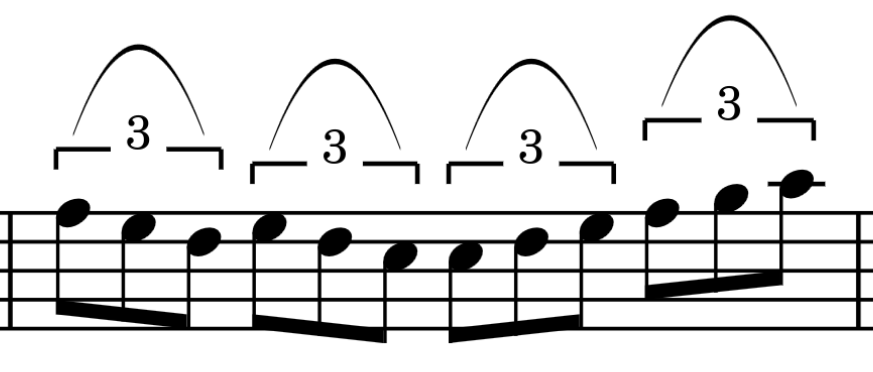
\includegraphics[width=.9\linewidth]{songs/flat-skareda-legata.png}
  \captionof{figure}{Nevzhledná legata nad triolami v programu \prog{Flat}. \prog{MuseScore} sází trioly pod trámci bez svorek.}
  \label{fig:flat-hnus}
\end{minipage}%
\hfill{}
\begin{minipage}{.45\textwidth}
  \centering
  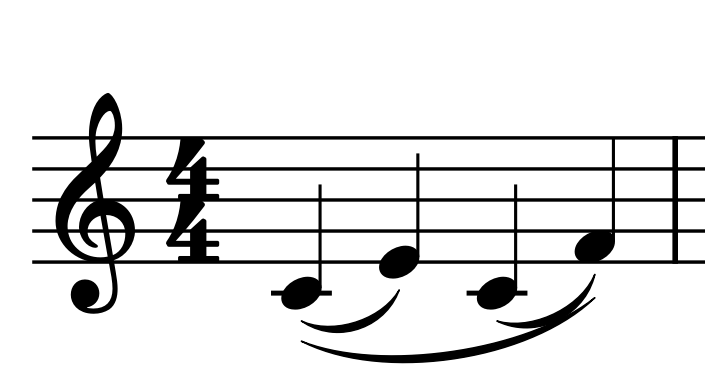
\includegraphics[width=.8\linewidth]{songs/musescore-kolize-.png}
  \captionof{figure}{Kolize dvou legat v \prog{MuseScore}. Legata se v tomto případě lehce dotýkají, nikdy se ale nepřekrývají.}
  \label{fig:muse-kolize}
\end{minipage}
%\end{figure}


% EDIT toto zdá se není pravda nakonec
% a i kdyby možná někdy, je to zbytečný nitpick protože MusiXTeX toto ani nepodporuje
%ale již neřeší jejich vzájemný překryv. Jejich kolize lze řešit ručním posunutím, což ale při častém používání vede k~nekonzistentnímu formátování.

\paragraph{Export části skladby}
\prog{MuseScore} ani \prog{Flat} neumožňují exportovat výběr dokumentu do grafického formátu~\cite{muse8yearsago}. Nelze tedy například vzít část skladby a zahrnout ji jako obrázek do jiného dokumentu; stránku je třeba ručně oříznout grafickým editorem.
 

\section{Balík \prog{MusiX\TeX}} % asi bych ponechal
\label{sec:musixtex}
\prog{MusiX\TeX{}} obsahuje sadu maker a písem umožňujících sazbu hudby v~systému \TeX{}. Zahrnuje symboly osnov, not, trámců, linek a dalších značek. \prog{MusiX\TeX{}} na základě posloupnosti \TeX{}ových maker určuje umístění jednotlivých prvků v~rámci partitury. Na rozdíl od sazby lineárního textu umožňuje práci s~několika notovými osnovami současně, což mimo jiné komplikuje řešení velikosti mezer mezi notami.

\prog{MusiX\TeX{}} kvůli řešení zalamování řádků zpracovává vstupní soubory třemi průchody. V~prvním průchodu zpracuje vstupní soubor příkazem \texttt{etex} a poznačí si rozestupy taktů do souboru s příponou \texttt{.mx1}. Ve druhém průchodu procesor \texttt{musixflx} řeší optimální velikost rozestupů not a výstup zapisuje do souboru s příponou \texttt{.mx2}. Ten je následně zahrnut ve finálním průchodu \texttt{etex}em. 

Zdrojový kód pro zahrnutí do \LaTeX{}ového dokumentu, který po sestavení zobrazuje úryvek Mozartovy Sonáty C-dur, vypadá následovně~\cite{musixtexdoc}:

\verbatimspace{}
\begin{verbatim}
\begin{music}
\parindent10mm
\instrumentnumber{1}        % 1 nástroj
\setname1{Piano}            % pojmenovaný Piano
\setstaffs1{2}              % se 2 notovými osnovami
\generalmeter{\meterfrac44} % 4/4 taktové označení
\startextract               % začátek úryvku
\Notes\ibu0f0\qb0{cge}\tbu0\qb0g|\hl j\en
\Notes\ibu0f0\qb0{cge}\tbu0\qb0g|\ql l\sk\ql n\en
\bar
\Notes\ibu0f0\qb0{dgf}|\qlp i\en
\notes\tbu0\qb0g|\ibbl1j3\qb1j\tbl1\qb1k\en
\Notes\ibu0f0\qb0{cge}\tbu0\qb0g|\hl j\en
\zendextract               % konec úryvku
\end{music}
\end{verbatim}
\verbatimspace{}
V úryvku mezi příkazy \verb+\startextract+ a \verb+\zendextract+ se jednotlivé noty uvádí po řádcích mezi makry \verb+\Notes+ a \verb+\en+. Nejprve je uvedena část not (ne nutně celý takt) pro spodní hlas (levou ruku), poté svislice \verb+|+ a následně odpovídající noty pro horní hlas (pravou ruku).
\newpage
\noindent 
Vysázené dílo poté vypadá takto:

\begin{figure}[h]
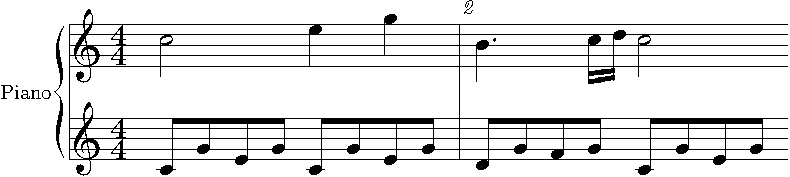
\includegraphics[width=\textwidth]{songs/sonata-crop.pdf}
\end{figure}

% Preprocesory
\section{Preprocesory pro \prog{MusiX\TeX}}
\label{sec:preprocesory}
Popis not \prog{MusiX\TeX}ovými makry je poměrně zdlouhavý a u~rozsáhlejších skladeb poněkud nečitelný.
Namísto přímého psaní maker lze notový vstup psát ve zkráceném formátu
a následně jej přeložit na prostý \TeX{}ový soubor obsahující jednotlivá \prog{MusiX\TeX}ová makra. Konkrétně lze k tomu využít jeden z preprocesorů, buď preprocesor \prog{PMX} nebo z něj vycházející procesor \prog{M-Tx}.


\subsection{Preprocesor \prog{PMX}}
Vstup preprocesoru \prog{PMX} se zapisuje do odděleného souboru s~příponou \texttt{.pmx}. \TeX{}ový výstup lze generovat příkazem \texttt{pmxab}, snadnější je však zdroje sestavovat obalujícím luaskriptem \texttt{musixtex}, který ve výchozím chování dokument přímo vysází do formátu \texttt{.pdf}.

Výslednou partituru ve formátu \texttt{ps} nebo \texttt{pdf} pak lze použít samostatně nebo zahrnout do jiného dokumentu \LaTeX{}ovým příkazem \verb"\includegraphics" jako vektorovou grafiku. Protože má však vysázená skladba rozměry celé strany, je žádoucí ji před zahrnutím oříznout -- buď ruční specifikací přes možnost \texttt{trim}, nebo automaticky například externím nástrojem \texttt{pdfcrop}.

% předtím je však vhodné výstup oříznout například příkazem \texttt{pdfcrop}.

Preambule vstupního souboru \texttt{.pmx} je velmi minimální.
Začíná posloupností 12 čísel, které určují parametry celé partitury. Popisují například počet notových osnov, nástrojů, definice taktových označení nebo počet stran. Následuje
seznam jmen nástrojů a určení klíčů pro jednotlivé osnovy.
Poslední řádek preambule tvoří adresářová cesta, do které má být zapsán
\TeX{}ový výstup \cite{pmxdoc}. Celá preambule včetně komentářů může vypadat například takto:

\verbatimspace{}
% lepší než zkratkovité instrukce
% nv,noinst,mtrnuml,mtrdenl,mtrnmp,mtrdnp,xmtrnum0,isig,
% npages,nsyst,musicsize,fracindent
\begin{verbatim}
% počet osnov, nástrojů, 4/4 takt, označený C, délka předtaktí,
       2          1         4 4        0 6           0    
% předznamenání, počet stran, řádků, velikost, předsazení
        0             1         1       20        0.07
Piano
bt
./
\end{verbatim}
\verbatimspace{}
% \newcommand{lit}[1]{\texttt{#1}}

% ($2\sim1/2$, $4\sim1/4$, $8\sim1/8$, $1\sim1/16$)
Tělo vstupního souboru \prog{PMX} poté určuje výšky a délky jednotlivých not. Noty se
zapisují písmeny \texttt{a-g}, následovanými číslicemi určujícími
délku (\mbox{\texttt{0} \semibreve}, \mbox{\texttt{2} \minim}, \mbox{\texttt{4} \crotchet}, \mbox{\texttt{8} \quaver}, \mbox{\texttt{1} \semiquaver}, \mbox{\texttt{3} \demisemiquaver}) a oktávu. Oddělení taktů svislou čarou není povinné, ale usnadňuje
kontrolu chyb. Dalšími příkazy lze přidávat posuvky (\texttt{s}\sharp, \texttt{f} \flat, \texttt{n} \natural), dynamiku a další značky. Oproti balíku \prog{Musix\TeX{}} je většina příkazů zkrácena na jeden znak, což zmíněný úryvek Sonáty C-dur zkracuje na pouhé dva řádky (zarovnání mezerami zde nehraje roli):
\verbatimspace{}
\begin{Verbatim}[samepage=true]
c83 g83 e g c83 g83 e  g | c83 g83 f g     c83 g83 e g /
c25         e4      g4   | bd-       c1 d1 c2          /
\end{Verbatim}
\verbatimspace{}
Délku not i oktávu si preprocesor udržuje podle předchozí noty, lze je tedy místy vynechat. U větších intervalových skoků je nutné uvést konkrétní oktávu absolutně číslem nebo relativně symboly \texttt{+}/\texttt{-}. Poněkud neintuitivní je u \prog{PMX} zápis hlasů v obráceném pořadí -- levý hlas klavíru je v tomto příkladu popsán horním řádkem.


% M-Tx
\subsection{Preprocesor \prog{M-Tx}}
Ve starších verzích procesor \prog{PMX} nepodporoval sazbu textů písní. V~současné verzi lze texty písní v~\prog{PMX} psát v~uvozovkách, které jsou poté obaleny do \TeX{}ového makra \texttt{pmxlyr}, dále rozvíjeného na \prog{MusiX\TeX} ové příkazy.

Alternativní rozhraní pro sazbu textů nabízí preprocesor \prog{M-Tx} (z anglického "Music from
Text")~\cite{mtxdoc}. Formát souboru \prog{M-Tx} je založen na formátu \prog{PMX}; podstatněji se liší ve
formátu preambule, kde místo seznamu hodnot používá seznam příkazů ve formátu
\texttt{Klíč:~hodnota}. Vstupní soubory se zpracovávají luaskriptem \texttt{musixtex}, který postupně volá jednotlivé procesory. Soubor je nejprve přeložen do formátu \texttt{.pmx}, poté zpracován preprocesorem \prog{PMX} a vysázen \TeX{}em. Oproti \prog{PMX} se zde jednotlivé osnovy zapisují v přirozeném vertikálním pořadí.

% Tady jsem si dovolil zkusit sazbu české písně a upozornit na vzniknuvší problémy, zároveň mi tato přijde mnohem uchopitelnější.

S ohledem na český text mi přišlo žádoucí zkusit sazbu českých písní včetně diakritiky. Bohužel, písmena s diakritikou nelze do \prog{MusiX\TeX{}}ových zdrojových souborů jednoduše zadávat. Částečné řešení, které umožňuje psát text s diakritikou v UTF-8, jsem přejal z dokumentace \prog{MusiX\TeX{}}u \cite[sekce 23.4]{musixtexdoc}. Spočívá ve změně kategorie písmen s diakritikou a následném překladu Lua\TeX{}ovým backendem. Takto lze text psát přirozenou češtinou:

\verbatimspace{}
\verbatiminput{songs/zachovej.mtx}
\verbatimspace{}

\noindent
%Překlad se poté provede následujícím příkazem:
%\verbatimspace{}
%\begin{verbatim}


%\footnote{V původním Varhanním doprovodu kancionálu jsou jednotlivé texty písní uvedeny přímo nad zápisem not pro varhany. M-Tx však neumožňuje doplňovat text ke spojeným hlasům, zpěv byl tedy vyčleněn do samostatného hlasu.}

Lua\TeX{}ový backend lze zvolit zadáním příslušného argumentu:
\verbatimspace{}
\begin{verbatim}
musixtex -F "luatex --output-format=pdf" soubor.mtx
\end{verbatim}
\verbatimspace{}
Vysázená skladba poté vypadá následovně:

\begin{figure}[H]
\centering
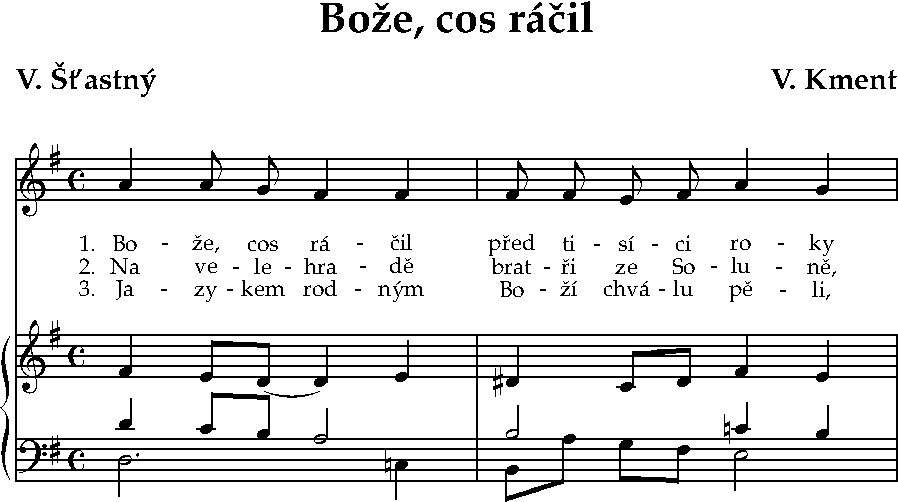
\includegraphics[width=0.9\textwidth]{songs/zachovej-crop.pdf}
\end{figure}


% NOTOVÉ ZNAČKY UVNITŘ TEXTU
\section{Notové značky uvnitř textu}
\label{sec:znacky}
Mimo sazbu not do notových osnov lze i psaný text doplnit notovými symboly, například pro
ilustraci hudební teorie. Symboly, které používá \prog{MusiX\TeX}, mají při použití v~textu nesprávnou velikost a nelze je tak do textu jednoduše začlenit.

Umístění hudebních značek do odstavců nabízí balíky \texttt{musicography} a~\texttt{lily\-glyphs}. Balík \texttt{musicography} má omezenější výběr, navíc jeho makra pro taktová označení kolidují s~těmi \prog{MusiX\TeX}ovými. 

Balík \texttt{lilyglyphs} využívá k~sazbě notových symbolů glyfy písma Emmentaler z~programu \prog{LilyPond}. K~vyhledání  % toto je fakt špatný nitpick
jednotlivých glyfů přitom závisí na balíku \texttt{fontspec}, díky čemuž vyžaduje k~překladu Lua\LaTeX. Pro porovnání vzhledu notových značek z obou balíků vizte tabulku~\ref{tab:comparison}.

%%%%%% TABULKA %%%%%%%%
\begin{table}[H]

\centering
\fbox{\begin{tabular}{l l l}


%musicography
Noty \musWhole\, \musHalf\, \musQuarter\, \musEighth\, \musSixteenth, &posuvky \musSharp\, \musFlat\, \musNatural, &taktová označení \musMeter{3}{4}\, \musMeter{4}{4}\, \musMeter{6}{8}\, \musMeterC\, \musMeterCutC. \\

% lilyglyphs
Noty \semibreve\, \minim\, \crotchet\, \quaver\, \semiquaver, &posuvky \sharp\, \flat\, \natural, &taktová označení \lilyTimeSignature{3}{4}\,  \lilyTimeSignature{4}{4}\, \lilyTimeSignature{6}{8}\, \lilyTimeC\, \lilyTimeCHalf\,.  \\

\end{tabular}}

\caption{Porovnání vzhledu a rozestupu některých symbolů z balíků \texttt{musicography} (nahoře) a \texttt{lilyglyphs} (dole) při
    oddělování mezerami \texttt{\textbackslash thinspace = \textbackslash ,}. Vysázené prvky z jednotlivých balíků mají odlišné mezery, taktová označení \texttt{musicography} mají pouze základní vzhled. 
}
\label{tab:comparison}
\end{table}
%%%%%% KONEC TABULKY %%%%%%%

Zahrnutí balíku \texttt{lilyglyphs} konkrétně u~šablony \texttt{csbulletin} zahlásí chybu při
duplicitní definici \texttt{centerbox}u. Jako workaround lze makro \texttt{centerbox} před načtením balíku \texttt{lilyglyphs} oddefinovat příkazem \verb"\let\centerbox\relax". Zároveň je u této šablony první z taktových označení \texttt{lilyglyphs} mírně nezarovnané, konkrétní příčinu jsem již ale nedohledal.


% NEDOSTATKY TEXOVÝCH SYSTÉMŮ
\section{Nedostatky \TeX{}ových systémů}
\label{sec:nedostatky}
V~porovnání s~konvenčními WYSIWYG editory jsou současné \TeX{}ové systémy poměrně obtížné. 
Začínající uživatele může odradit nedostatek zdrojů, často omezený na oficiální dokumentace, které jsou často příliš dlouhé nebo neobsahují dostatek názorných příkladů. Názornější mohou být příklady skladeb a dodatečné příručky dostupné z~webu~\textit{Werner Icking Music Archive}~\cite{wima}, konkrétně například návod \textit{Typesetting Music With \prog{PMX}}~\cite{pmxtutorial}.

Dalším nedostatkem \TeX{}ových systémů a jejich preprocesorů jsou místy nečitelné chybové zprávy. Jako příklad uvádím zprávu, která může uživatele zaskočit při zpracování souboru \prog{PMX} s nesprávným formátem hlavičky. Hlášení v~tomto případě nevypisuje kód \prog{PMX}, ale přímo formátovací funkce Fortranu, ve kterém je \prog{PMX} implementován~\cite{pmxdoc}. Každopádně hledání příčiny problému příliš neusnadňuje:

\verbatimspace{}
\begin{verbatim}
fmt: read unexpected character
apparent state: internal I/O
last format: (f1.0)
lately reading sequential formatted internal IO
\end{verbatim}
\verbatimspace{}

Mimoto je také možné, že samotná podstata textové sazby nemusí být pro řadu uživatelů zcela intuitivní, což může bránit širšímu rozšíření těchto nástrojů.



\subsection{Program LilyPond}
Alternativu k~\TeX{}ovým makro balíkům může představovat program \prog{LilyPond}. Na rozdíl od
představených procesorů není vázán na \TeX{} a existují k~němu grafické editory, například \prog{Frescobaldi} či \prog{Denemo}. Zatímco Frescobaldi ze zadaného zdrojového kódu generuje náhled skladby, Denemo umožňuje naopak noty vkládat interaktivně a zpětně generuje kód pro LilyPond~\cite{lily-frontend}.

Kód LilyPondu lze zahrnout i do \TeX{}ových souborů, konkrétně buďto inline prostřednictvím makra \texttt{lilypond}
nebo častěji přes stejnojmenné prostředí:

\verbatimspace{}
\begin{verbatim}
\begin{lilypond}[quote,fragment,staffsize=26]
  c' d' e' f' g'2 g'2
\end{lilypond}
\end{verbatim}
\verbatimspace{}

% odstraněno, protože jsem to vlastně sám nezprovoznil
%Pro překlad dokumentu existují dvě možnosti. V případě sazby příkazem \texttt{lilypond-book} tato prostředí \LaTeX{} vůbec nezpracovává, \prog{LilyPond} tyto sekce předem vysází a následně zahrne do souboru jako obrázek namísto těchto prostředí a poté až následuje samotný překlad \LaTeX{}em. 

Pro překlad dokumentu lze použít makrobalík \textit{LyLua\TeX{}} krátce představený v minulém čísle Zpravodaje~\cite[sekce~5]{vysokourovnovejazyky}. Po zahrnutí příkazem \texttt{\textbackslash usepackage\{ly\-lua\-tex\}} lze sázet dokument přímo příkazem \texttt{lualatex}:

\verbatimspace{}
\begin{verbatim}
lualatex --shell-escape document.tex
\end{verbatim}
\verbatimspace{}

Vysázený úryvek poté vypadá takto. Pokud je cílem uvést úryvek do jiného dokumentu (jako zde) a využívá se pro ořez \texttt{pdfcrop}, je potřeba vypnout \LaTeX{}ové číslování stran příkazem \texttt{\textbackslash pagenumbering\{gobble\}}.
\begin{figure}[H]
    \centering
    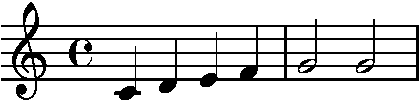
\includegraphics[width=.4\textwidth]{songs/lily-crop.pdf}
    \label{fig:lily-crop}
\end{figure}


\let\addspace\biblatexaddspace

\printbibliography

% KONEC
\begin{summary}
\TeX{} is a useful tool for text typesetting; however, it doesn't feature a good support for composition typesetting at its core. The TUG 2022 conference featured a talk on notation typesetting which compared the \prog{MusiX\TeX{}} package with the \textit{MuseScore} and \textit{Flat} tools, but did not mention the \prog{PMX} and \prog{M-Tx} preprocessors. 
In this article, I compare typesetting using \prog{MusiX\TeX{}} and its preprocessors and describe its usage. In addition, I describe the incorporation of note symbols into a paragraph text. 
After reading the article, the reader will be able to create a short simple excerpt of a piece of music and incorporate it into a \TeX{} document, as well as add musical symbols to a written text.
\keywords:sheet music, music engraving, \prog{MusiX\TeX}, \prog{PMX}, \prog{M-Tx},  \prog{LilyPond}, \prog{MuseScore}, \prog{Flat}
\end{summary}

\end{document}
